\section{Problem Statement}
\label{sec:problemStatement_IK}

In this chapter, we focus on the problem of user input manipulation by a compromised host PC in scenarios such as the web-based remote configuration of safety-critical devices, financial transitions, emails, and social media posts. (Attacks that compromise safety-critical systems directly are discussed in the literature; a survey of such works can be found in~\cite{fachkha2017internet}.)


%In social media, manipulation of articles is also widespread~\cite{gordon,fitzpatrickmedia}.

\subsection{System Model}

\begin{figure}[t]
    \centering
    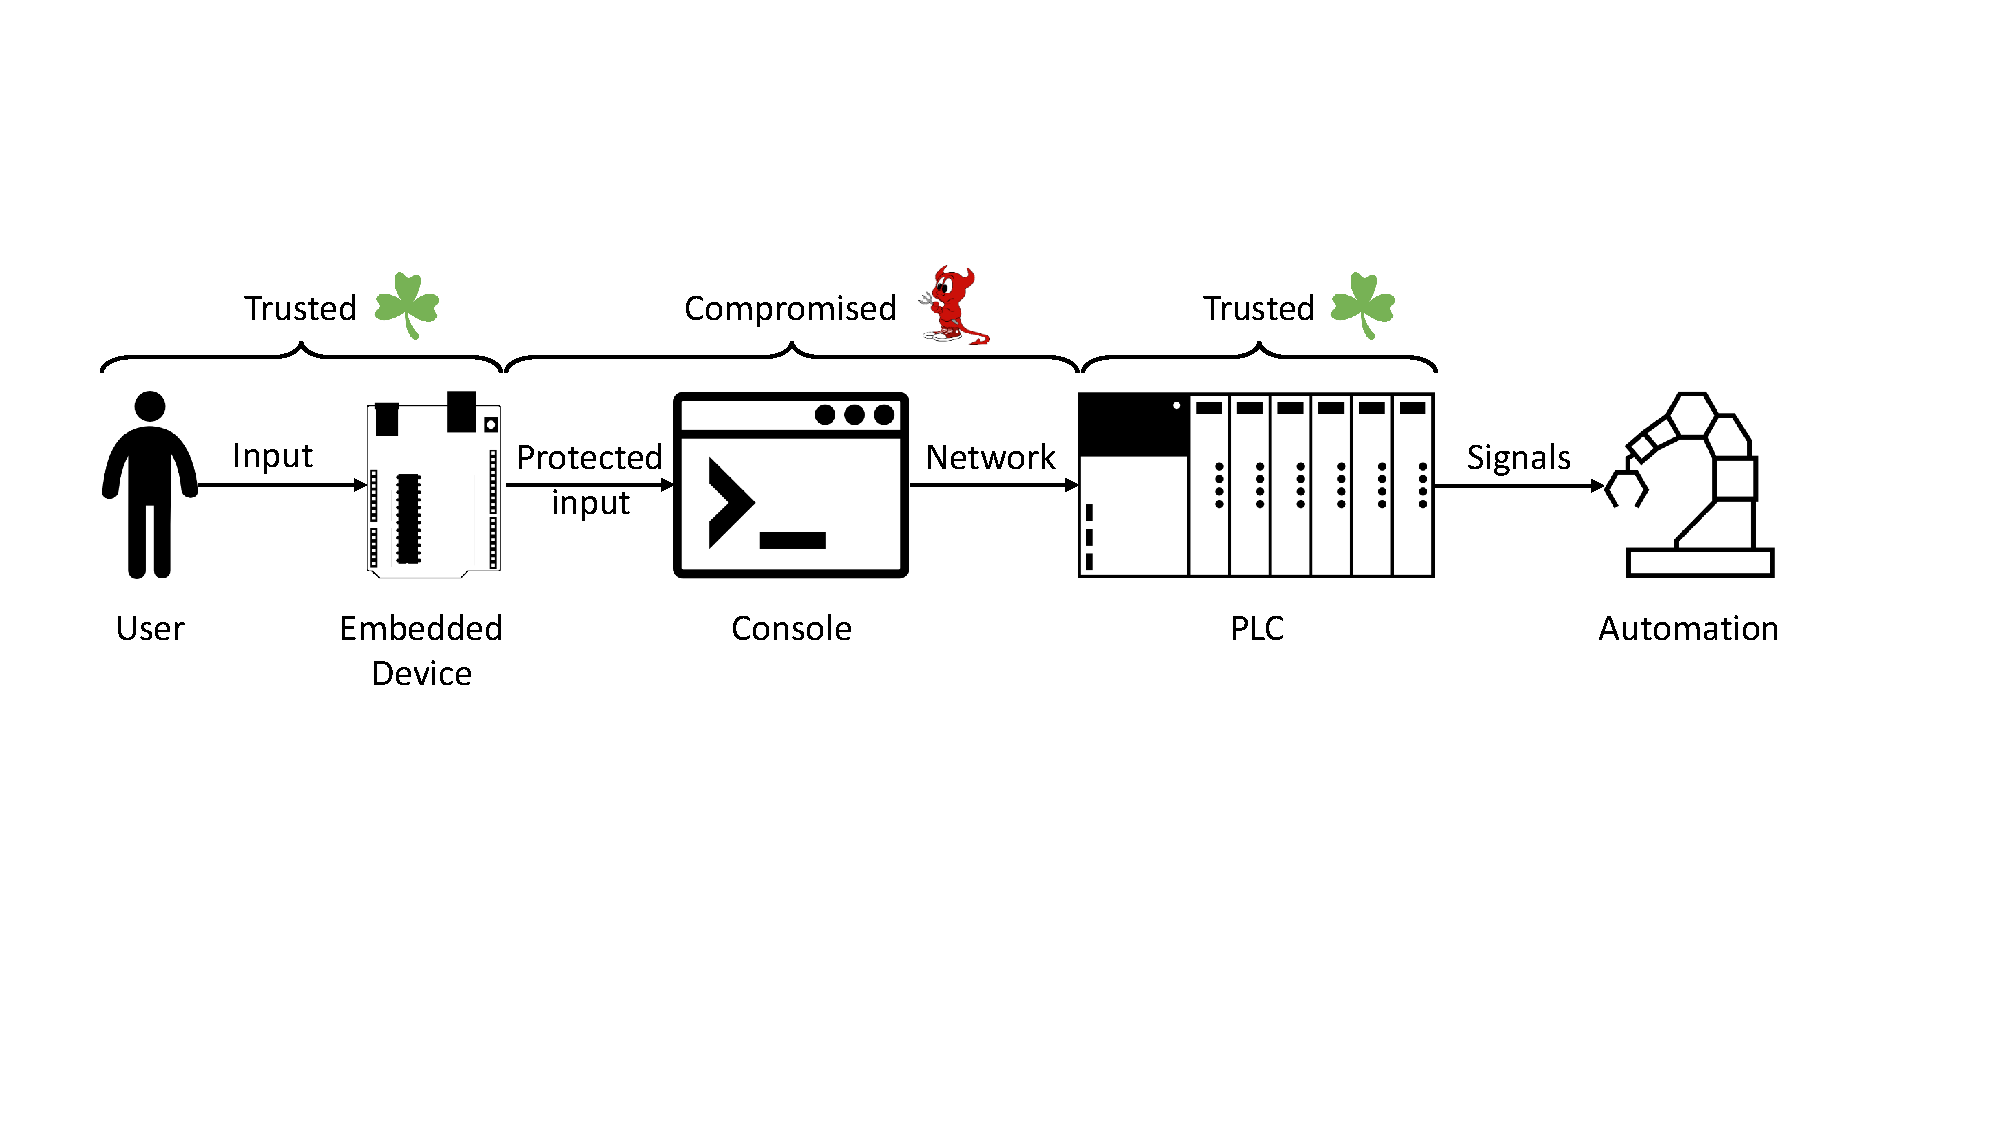
\includegraphics[trim={0 8cm 14cm 0},clip,width=0.9\linewidth]{chapters/IntegriKey/images/Motivation.pdf}
    %\caption{\textbf{System model.} We consider a setting where the user configures a safety-critical device through a web service from untrusted localhost. The user input device (keyboard) and the target safety-critical device are trusted. The host platform and the network connection can be controlled by the attacker.} 
    \caption[System model for remote safety-critical services through an attacker-controlled host]{\textbf{System model for remote safety-critical services through an attacker-controlled host.} We consider a setting where the user configures a safety-critical device or executes financial transactions through a web service from untrusted localhost. The user input device (keyboard) and the end-system (target device, bank server, medical implants, etc.) are trusted. The host platform and the network connection can be controlled by the attacker.} 

    \label{fig:systemModel}
\end{figure}

Our system model is illustrated in Figure~\ref{fig:systemModel}. We consider a common setting, where the user interacts with a security-critical web interface that, for example, configures a safety-critical device like a medical device, industrial robot, or home automation system or executes financial transactions over the Internet. The user provides input through an input device (in our case keyboard) to a web browser running on the \emph{host} machine that is a standard PC. The browser sends the configuration input to a \emph{server} that configures (or is) the safety-critical device.

We focus on \emph{keyboard} input, as such input is sufficient to use the configuration web interfaces of many existing safety-critical devices~\cite{7306669,controlbyweb,siemens,siemens2,schneider} and online wallets \cite{bitgo,bitcoinwallet,coin,blockchain,coinbase}. Later in this chapter, see Section~\ref{sec:discussion}, we discuss the challenges of protecting other types of input devices, such as mouse input, with the same approach.

\myparagraph{attacker model} We consider the user input device (i.e., the keyboard) trusted and the target safety-critical device, and the server that receives the user input also trusted. We assume that the attacker may have remotely compromised the host platform completely, i.e., the attacker controls the operating system, the browser, and any other software running on the host. We consider that even the host hardware can be exploitable. We assume that the attacker does not have physical access to the host platform.

We consider such strong attacker realistic since OS vulnerabilities in PC platforms are well-known, browser compromise is increasingly common (see, e.g.,~\cite{provos2007ghost,dougan2012man} for recent attack vectors), and hardware exploits are possible, e.g., through fabrication-time attacks~\cite{Lin2009,a2}. 

\subsection{Limitations of Known Solutions}

The problem of trusted user input to a remote server through an untrusted host has been studied in a few different contexts. Here we review the main limitations of known approaches, while Section~\ref{sec:relatedWork_IK} provides a more extensive review of related work.

\myparagraph{Transaction confirmation} One common approach is transaction confirmation using a separate trusted device. For example, in the ZTIC system~\cite{weigold2011}, a USB device with a small display and limited user input capabilities are used to confirm transactions such as payments. The USB device shows a summary of the transaction performed on the untrusted host, and the user is expected to review the summary from the USB device display before confirming it. Proposals such as Phoolproof~\cite{parno2006phoolproof} uses a second device such as a smartphone as a second factor for visiting website to mitigate phising attack. This approach is prone to \emph{user habituation}, i.e., the risk that users confirm transactions without carefully examining them to be able to proceed with their main task, such as completing the payment, similar to systems that rely on security indicators~\cite{schechter2007emperor,197283,41927}. Another limitation of this approach is that it breaks the normal workflow, as the user has to focus his attention on the USB device screen in addition to the user interface of the host. Finally, such trusted devices with displays and input interfaces can be expensive to deploy. 

\myparagraph{Trusted hypervisor} Another common approach is secure user input using a trusted hypervisor. Gyrus~\cite{gyrus} and Not-a-Bot (NAB)~\cite{nab} are systems where a trusted hypervisor, or a trusted VM, captures user input events and compares them to the application payload that is sent to the server. SGXIO~\cite{weiser2017sgxio} assumes a trusted hypervisor through which the user can provide input securely to a protected application implemented as an Intel SGX enclave~\cite{sgx} which in turn can securely communicate with the server. The main limitation of such solutions is that even minimal hypervisors have large TCBs, and vulnerabilities are often found in them~\cite{hashizume2013analysis,perez2013characterizing}.

\myparagraph{Dynamic root of trust} The third common approach is trusted user input using \emph{dynamic root of trust}~\cite{mccune2008flicker}. In the UTP system~\cite{filyanov2011uni}, the normal execution of the OS is suspended, and a small \emph{protected application} is loaded for execution. The protected application includes a minimal display and keyboard drivers and is, therefore, able to receive input from the user and send it to the server together with a remote attestation that proves the integrity of the application handling the user input. The main drawback of this approach is that it changes the user experience of the web-based configuration application significantly, as small protected applications cannot implement complete web UIs. For example, the UTP system implements only a minimal VGA driver for text-based user interfaces.


\subsection{Design Goals}

Given these limitations of previous approaches, our solution has the following main design goals: 

\begin{enumerate}
    \item \emph{Strong integrity protection.} Our solution should provide strong user input integrity protection even if the input host and the network are compromised. In particular, the solution should have a small TCB and not rely on tasks like transaction confirmations which are prone to user habituation. 

    \item \emph{Easy deployment.} Our solution should be easy to deploy. In particular, we want to avoid significant changes to existing safety-critical systems, input devices, host platforms, or the web-based remote configuration user experience. We also want to avoid the deployment of expensive hardware.
\end{enumerate}




